%!TEX root = ../dokumentation.tex

\chapter{Umsetzung}

Im folgenden wird nun detailliert auf das entwickelte Konzept eingegangen und deren Funktionsweisen erläutert.

%title wird unter dem Bsp. abgedruckt
%caption wird im Verzeichnis abgedruckt
%label wird zum referenzieren benutzt, muss einzigartig sein.

\section{Voraussetzungen}
Für die Nutzung des Audioplayer auf dem Raspberry Pi bzw. für die weitere Entwicklung, müssen vorerst einige Anpassungen und Installationen getätigt werden. Diese Schritte sind notwendig damit der Audioplayer wie vorgesehen funktioniert und keine unvorhergesehen Zustände entstehen.

\subsection{Pakete installieren und Raspberry Pi updaten}
Standardmäßig besitzt der Raspberry Pi das Betriebssystem \textit{Raspbian}. Dieses gilt es zuerst auf die neuste Version zu aktualisieren. Zusätzlich werden alle installierten Pakete des System auf die neuste Version zu aktualisieren. Dieses Vorhaben wird mit den folgenden Befehlen durchgeführt:
\begin{lstlisting}[caption={Aktualsierien des Raspberry Pi}]
sudo apt-get update 
sudo apt-get upgrade 
sudo apt-get install rpi-update 
sudo rpi-update
\end{lstlisting}
Die ersten drei Befehle werden mit \ac{APT} ausgeführt. \ac{APT} ist ein Paketverwaltungssystem welches für den Bereich der Debian Betriebssysteme entwickelt wurde. Das Tool verwaltet Debian Pakete und somit auch die installierten Applikationen auf dem Raspberry Pi \autocite{apt-debian-wiki_2019}.
Zusätzlich wird für alle durchzuführende Befehle der \textit{sudo} Befehl benutzt. \ac{Sudo} wird meistens dafür benutzt bestimmte Befehle mit Root-Rechten also mit Administratorrechten auszuführen. Der Vorteil liegt darin, dass der Nutzer eben nicht ein Administrator sein muss, um kurzfristig einen Befehl als Administrator auszuführen \autocite{moeller_2013}.
Mit dem Befehl \textit{sudo apt-get update} werden alle Paketquellen neu eingelesen - also ein großes Lexikon wo man jedes Paket mit der neusten zur Verfügung stehenden Version finden kann.
Mit dem Befehl \textit{sudo apt-get upgrade} werden alle bereits installierten Paket auf die in den Paketquellen vorhandene neuste Version aktualisiert. Dabei werden keine neuen Pakete installiert oder alte nicht mehr benötigte Abhängigkeiten entfernt. \autocite{apt-get-wiki_2019}
Mit dem Befehl \textit{apt-get install rpi-update} wird das Paket \textit{rpi-update} mit allen seinen Abhängigkeiten heruntergeladen und installiert. Das Paket ist ein automatisiertes Skript zum updaten des Raspberry Pi's Betriebssystem auf die neuste Version.
Als letzten Schritt wird nun das Paket \textit{rpi-update} ausgeführt und der Raspberry Pi lädt automatisch das neuste passende Betriebssystem herunter und installiert es. Dabei gehen keine Daten verloren.
\\
Nachdem der Raspberry Pi sich erfolgreich aktualisiert hat, müssen nun noch die jedenfalls benötigten Pakete installiert werden. Dies wird mit den folgenden Befehlen gemacht.
\begin{lstlisting}[caption={Installation benötigter Pakete}]
sudo apt-get install portaudio19-dev
sudo apt-get install libmpg123-dev
sudo apt-get install mp3info 
\end{lstlisting}

\subsection{Nötige Schritte für Entwicklungszwecke}
Im folgenden wird auf die einzelnen Schritte eingegangen, die nötig sind um an dem erstellten Programm weiter zu entwickeln. Dazu müssen die im Anschluss stehenden Befehle auf dem Raspberry Pi ausgeführt werden.
\subsubsection{Installieren von Go}
Nun wird auf die Installation von Go eingegangen.
\begin{enumerate}
\item \textbf{Herunterladen von Go}  \\
Link: https://golang.org/dl/ \\
Kind: Archive \\
OS: Linux \\
Arch: ARMv6
\begin{lstlisting}
Befehl: wget [LINK]
\end{lstlisting}

\item \textbf{Entpacken des Archivs}  \\
\begin{lstlisting}
tar -C /usr/local -xzf [Filename]
\end{lstlisting}

\item \textbf{Setzen des Export-Pfad} \\
\begin{lstlisting}
export PATH=\$PATH:/usr/local/go/bin
\end{lstlisting}

\item \textbf{Überprüfen der Go Installation auf Korrektheit} \\
\begin{lstlisting}
go version -> "go version go x.x.x"
\end{lstlisting}

\item \textbf{Go-Ordnerstruktur anlegen} \\
\textbf{bin} will contain all Go executable's you have installed using go install command. \\ 
\textbf{pkg} will contain all compiled packages that can be imported into your projects. 
\\
\textbf{src} will contain all your source files, either your own or sources downloaded from external repositories. \newline
Der Ordner \textit{pi} stellt hier den Nutzernamen da, der sich bei jedem System natürlich unterscheiden kann. \\
\begin{minipage}[t]{\textwidth}
\dirtree{%
.1 /. 
.2 home. 
.3 pi. 
.4 go. 
.5 src. 
.5 pkg. 
.5 bin. 
}
Befehle zur Erstellung der Ordnerstruktur - Start bei \$Home:
\begin{lstlisting}[caption={Erstellung der Go Ordnerstruktur}]
mkdir go
cd go
mkdir src
mkdir pkg
mkdir bin
\end{lstlisting}
\end{minipage}


\end{enumerate}

\subsubsection{Klonen des Git Repository}
Der nächste Schritt ist das Git Repository auf den lokalen PC zu klonen. Go schreibt dafür einen standard vor, wie die Ordnerstruktur dazu aufgebaut werden sollte. Im folgenden ist nun die Ordnerstruktur und den dafür nötigen Code dargestellt. 
Diese Befehle Starten von /home/pi/go/src/ :
\begin{lstlisting}[caption={Klonen des Git Repository}]
mkdir github.com 
cd github.com
mkdir alexanderklapdor
cd alexanderklapdor
git clone https://github.com/alexanderklapdor/RaspberryPi_Go_Audioplayer.git
\end{lstlisting}

\subsubsection{Installieren der Go Abhängigkeiten}
Starting from ../RaspberryPi\_Go\_Audioplayer/ :
\begin{lstlisting}
go get ./...  
\end{lstlisting}

\subsubsection{Modifizieren der ALSA Bibliothek Dateien}
Die Konfigurationdatei der ALSA Bibliothek muss editiert werden damit die Fehlermeldungen, welche durch die nicht vorhandenen Anschlüsse am Raspberry Pi hervorgerufen werden, nicht immer mit ausgegeben werden. \\
Zugriff auf die Datei wird mit dem Befehl \textbf{sudo nano /usr/share/alsa/alsa.conf}  \\
Folgende Einträge müssen aus dieser Datei entfernt werden:
\begin{lstlisting}[caption={Liste der zu löschenden Einträge}]
pcm.rear cards.pcm.rear 
pcm.center_lfe cards.pcm.center_lfe 
pcm.side cards.pcm.side 
pcm.surround21 cards.pcm.surround21 
pcm.surround40 cards.pcm.surround40 
pcm.surround41 cards.pcm.surround41 
pcm.surround50 cards.pcm.surround50 
pcm.surround51 cards.pcm.surround51 
pcm.surround71 cards.pcm.surround71 
pcm.iec958 cards.pcm.iec958 
pcm.spdif iec958 
pcm.hdmi cards.pcm.hdmi 
pcm.dmix cards.pcm.dmix 
pcm.dsnoop cards.pcm.dsnoop 
pcm.modem cards.pcm.modem 
pcm.phoneline cards.pcm.phoneline
\end{lstlisting}

\subsection{Nötige Schritte für die Nutzung}
Für die reine Nutzung des Audioplayer sind durchaus weniger Schritte notwendig, da eine bereits kompilierte Version heruntergeladen und genutzt werden kann.
Dazu sind folgende Schritte notwendig:
\begin{enumerate}
\item \textbf{Herunterladen der neusten \href{https://github.com/alexanderklapdor/RaspberryPi_Go_Audioplayer/releases}{Release} Datei}  \\
\begin{lstlisting}
wget [LINK]
\end{lstlisting}

\item \textbf{Entpacken des Archiv} \\
\begin{lstlisting}
tar -xvf RaspberryPi_Go_Audioplayer_v***.tar
\end{lstlisting}

\item \textbf{Starten des Audioplayers} \\
\begin{lstlisting}
./RaspberryPi_Go_Audioplayer_v***/MusicPlayerClient
\end{lstlisting}
\end{enumerate}

\section{Konzept}
Hier wird das allgemeine/übergeordnete Konzept dargestellt. Das muss dann hier auch noch genau erläutert werden wie das funktioniert, mit dem Hinweis, dass auf die einzelnen Punkte wie Client, Server und Socket im nach hinein nochmals explizit eingegangen wird
\begin{figure}[h]
	\centering
	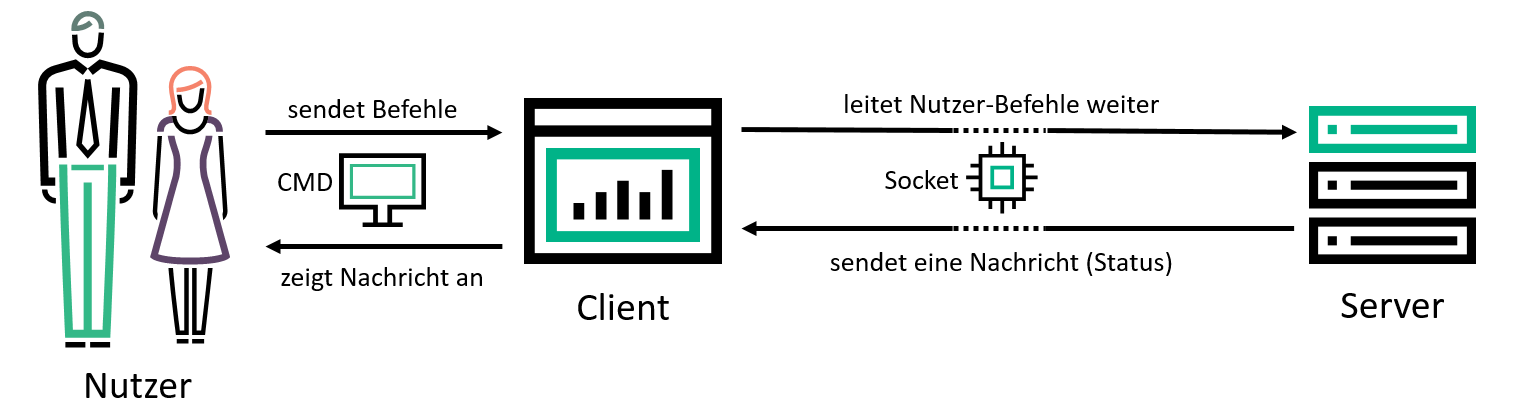
\includegraphics[scale=0.5]{Audioplayer_Konzept.png}
	\caption{Audioplayer - Konzept}
	\label{img:grafik-RaspberryPi3}
\end{figure}
\newline

\subsection{Konzept des Clients}
Hier kommt der Scheiß ist zustand rein

\begin{figure}[ht]
    \begin{struktogramm}(150,60)[Client Ablauf] 
        \assign{Konfigurationsdatei auslesen} 
        \assign{Aufsetzen des Loggers}
                        \ifthenelse[12]{1}{2} {Überprüfen ob Server bereits läuft}{Ja}{Nein} 
                        \assign{}
                        \change
                        \assign{Starten des Servers}
                        \ifend
                        \ifthenelse[12]{2}{1} {Überprüfen ob Übergabeparameter übergeben wurden}{Ja}{Nein} 
                        \assign{Parsen der Informationen in ein JSON Format}
                        \assign{Senden des JSONs and den Server}
                        \change
                        \assign{Beenden des Clients}
                        \ifend
    \end{struktogramm} 
\caption{Client Programm - Ablauf} 
\label{lst:client_ablauf} 
\end{figure}

\begin{figure}[h]
	\centering
	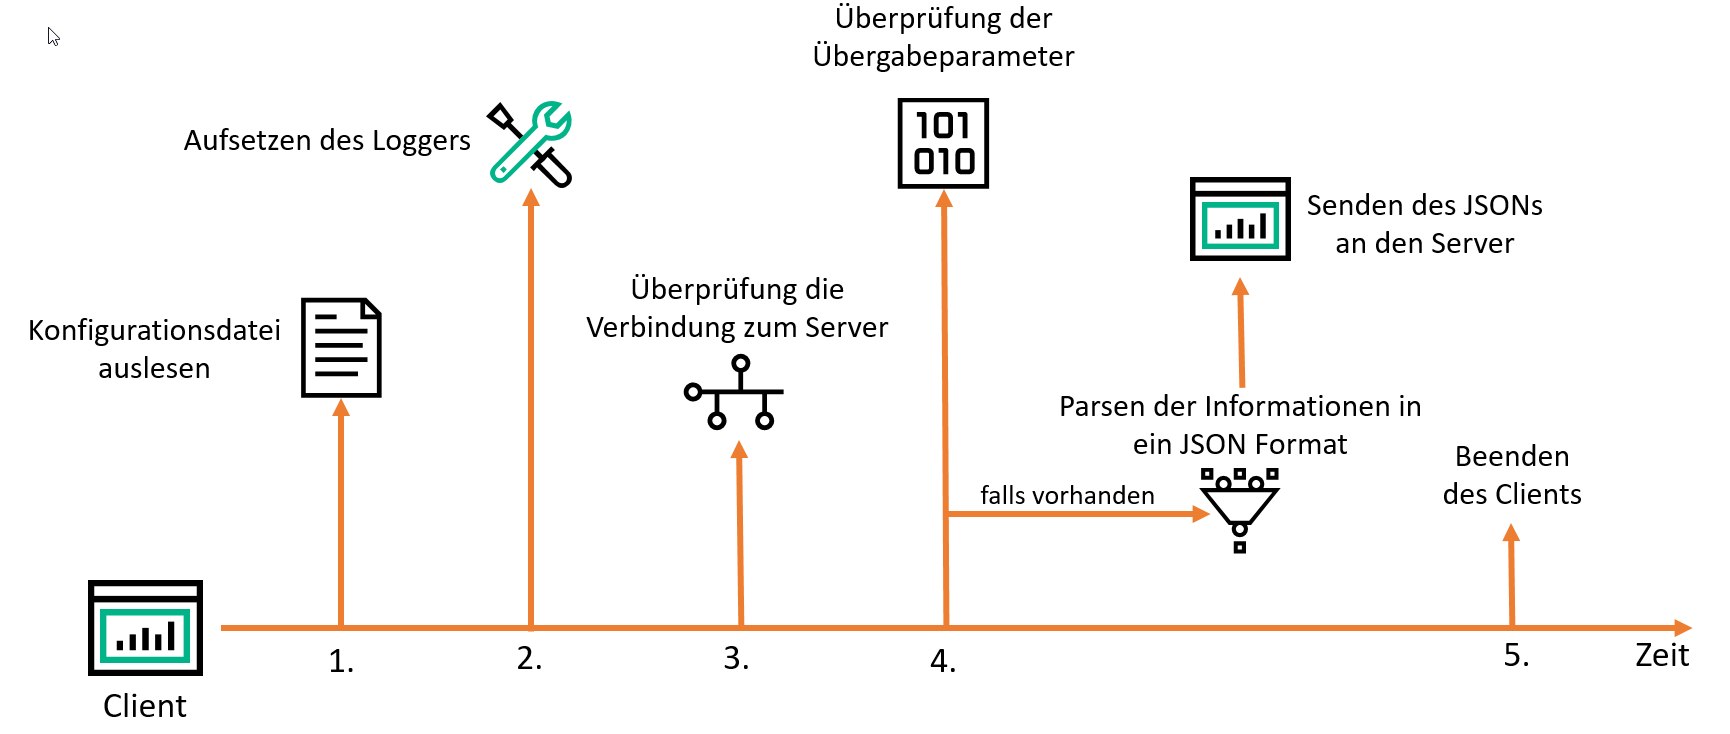
\includegraphics[scale=0.3]{Client_Konzept.png}
	\caption{Audioplayer - Konzept}
	\label{img:grafik-RaspberryPi3}
\end{figure}

1. Holt sich die Config(da stehen alle Sachen drinnen wie Ort des Sockets und blabla)\\
2. Setzt den Logger auf \\
3. Überprüft ob der Server bereits läuft, wenn nicht dann startet er den Server und wartet solange bis er hochgefahren ist und die Verbindung zum socket besteht. \\
4. Überprüft ob Übergabeparameter(Kommando) übergeben wurden. Wenn nicht dann Programm beenden, wenn doch dann Parsen den Übergabewerte \\
5. Packen der geparsten Informationen in ein JSON Format und senden dies JSON über den Socket an den Server. \\
6. Beenden des Clients \\

\subsection{Konzept des Servers}

1. Holt sich die Config(da stehen alle Sachen drinnen wie Ort des Sockets und blabla)\\
2. Setzt den Logger auf \\
3. Setzt den Socket auf \\
4. Starten Pulseaudio \\
5. Hört den Socket ab \\
	5.1 Falls nichts kommt...warten \\
	5.2 Falls was reinkommt - JSON Parsen und das gewünschte Kommando ausführen.\\
	

\section{Kommunikation über Sockets}
Sockets erklären und kurz erläutern warum wir die verwendet haben.\\
\\
Ein Socket (von engl. Sockel, Steckverbindung oder Steckdose) ist ein vom Betriebssystem bereitgestelltes Objekt, das als Kommunikationsendpunkt dient. Ein Programm verwendet Sockets, um Daten mit anderen Programmen auszutauschen. Das andere Programm kann sich dabei auf demselben Computer (Interprozesskommunikation) oder einem anderen, via Netzwerk erreichbaren Computer befinden. Die Kommunikation über Sockets erfolgt in der Regel bidirektional, das heißt, über das Socket können Daten sowohl empfangen als auch gesendet werden.

\section{Funktionen des Programms}
Hier kommen die Scheiß Funktionen rein, alle Beschreiben und vll. kurz erläutern evtl. an einer Zeichnung wie diese Ablaufen.

\href{https://github.com/alexanderklapdor/RaspberryPi_Go_Audioplayer#commands-of-the-client}{Kommandos}
\\
\href{https://github.com/alexanderklapdor/RaspberryPi_Go_Audioplayer#console-arguments}{Console-Arguments}


\section{Bedienung des Programms}
Beispiele für die Bedienung reinmachen ( Ordner abspielen, Loop, Playlist, blabla)

